\begin{figure*}[t]
    \centering
    \vspace{-10pt}
    \hspace{-25pt}
    % \hspace*{-2cm}
    ~ %add desired spacing between images, e. g. ~, \quad, \qquad, \hfill etc. 
      %(or a blank line to force the subfigure onto a new line)
            %\hspace{-20pt}
    \begin{subfigure}[b]{0.48\textwidth}
        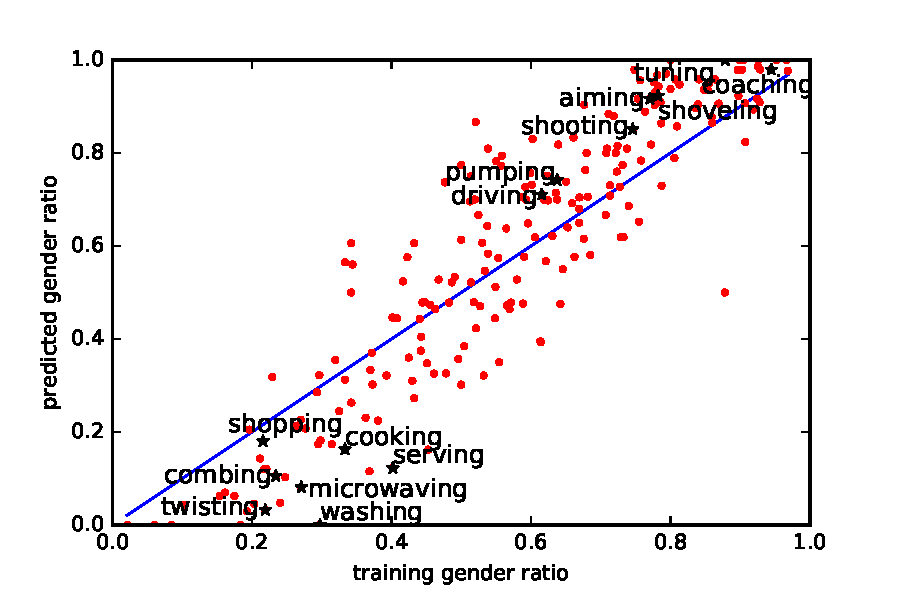
\includegraphics[width=1.15\linewidth]{figures/gender_ratio_dev.pdf}
        \caption{Bias analysis on imSitu vSRL}
        \label{fig:biased_verb_dev}
    \end{subfigure}
   % \hspace{-16pt}
  %  \begin{subfigure}[b]{0.26\textwidth}
  %      \includegraphics[width=\linewidth]{figures/gender_ratio_train.pdf}
  %      \caption{Gender ratio on training. }
  %      \label{fig:biased_verb_train}
  %  \end{subfigure}
    %~ %add desired spacing between images, e. g. ~, \quad, \qquad, \hfill etc. 
    %(or a blank line to force the subfigure onto a new line)
  %        \hspace{-20pt}
  %  \begin{subfigure}[b]{0.26\textwidth}
  %      \includegraphics[width=\linewidth]{figures/meanVerbRatio_for_man_dev.pdf}
  %      \caption{Verb distribution of ``men''.}
  %      \label{fig:verb_ratio}
  %  \end{subfigure}
  %        \hspace{-20pt}
    ~ %add desired spacing between images, e. g. ~, \quad, \qquad, \hfill etc. 
    %(or a blank line to force the subfigure onto a new line)
  %  \begin{subfigure}[b]{0.42\textwidth}
  %      \includegraphics[width=\linewidth]{figures/bias_score_each_verb_oridev_imSitu.pdf}
  %      \caption{Bias amplification across verb by confidence threshold, averaged across verbs.
  %       Values near zero indicate no bias amplification.
        %As the system becomes less confident, it amplifies bias more. Even at high confidence thresholds, bias amplification persists.
  %      }
   % \label{fig:bias_score_imSitu}
%    \end{subfigure}
   \begin{subfigure}[b]{0.48\textwidth}
        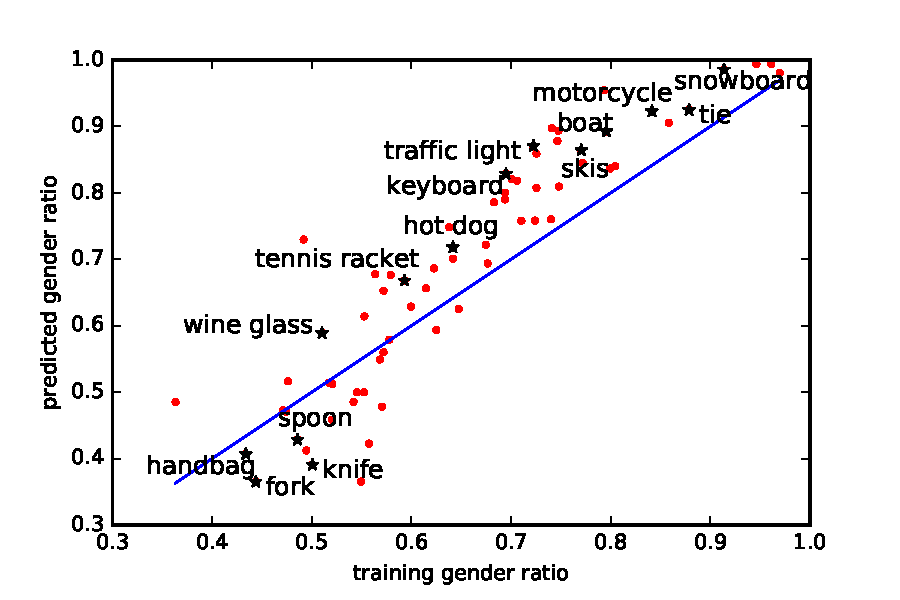
\includegraphics[width=1.15\linewidth]{figures/gen_ratio_obj_coco_test.pdf}
        % \caption{Gender bias of MS-COCO objects toward \texttt{man} in training set versus bias on a predicted development set. Values near zero indicate bias}
        \caption{Bias analysis on MS-COCO MLC}
        \label{fig:gen_dev_coco}
    \end{subfigure}
    \caption{Gender bias analysis of imSitu vSRL and MS-COCO MLC. (a) gender bias of verbs toward \texttt{man} in the training set versus bias on a predicted development set. (b) gender bias of nouns toward \texttt{man} in the training set versus bias on the predicted development set. Values near zero indicate bias toward \texttt{woman} while values near $0.5$ indicate unbiased variables. Across both dataset, there is significant bias toward males, and significant bias amplification after training on biased training data.}
    \label{fig:imSitu_results}
\end{figure*}

%\begin{figure*}[t]
%    \centering
    % \hspace*{-2cm}
    ~ %add desired spacing between images, e. g. ~, \quad, \qquad, \hfill etc. 
      %(or a blank line to force the subfigure onto a new line)
%    \begin{subfigure}[b]{0.42\textwidth}
%        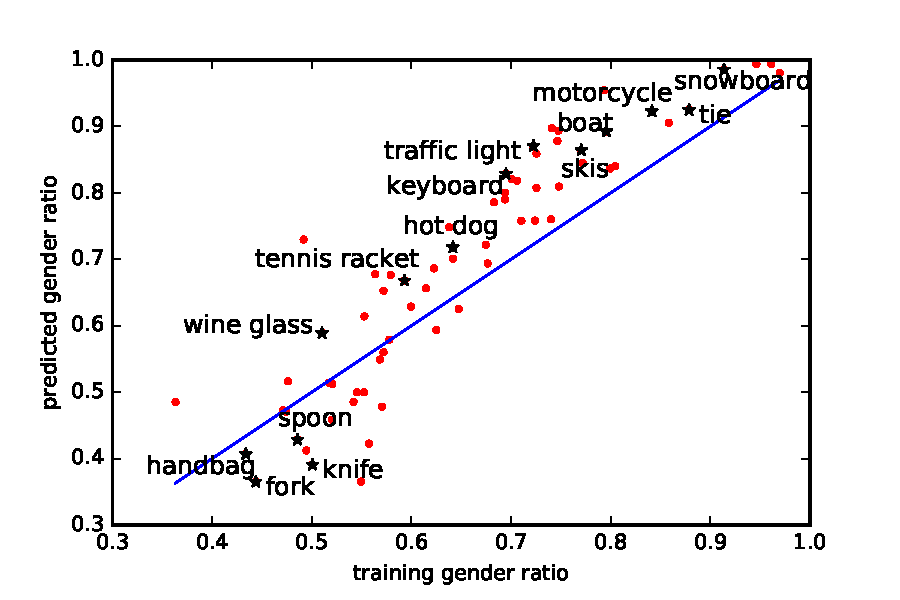
\includegraphics[width=\linewidth]{figures/gen_ratio_obj_coco_test.pdf}
%        \caption{Gender bias of MS-COCO objects toward \texttt{man} in training set versus bias on a predicted dev set.}
%        \label{fig:gen_dev_coco}
%    \end{subfigure}
   % ~
   %\hspace{-0pt}
%     \begin{subfigure}[b]{0.31\textwidth}
 %       \includegraphics[width=\linewidth]{figures/gen_ratio_obj_coco_train.pdf}
  %      \caption{Gender ratio on train. }
   %     \label{fig:gen_train_coco}
    %\end{subfigure}
    ~ %add desired spacing between images, e. g. ~, \quad, \qquad, \hfill etc. 
    %(or a blank line to force the subfigure onto a new line)
%    \begin{subfigure}[b]{0.42\textwidth}
%        \includegraphics[width=\linewidth]{figures/gen_ratio_super_coco.pdf}
%        \caption{Gender bias of  MS-COCO object toward man, grouped by object super-categories.}
%        \label{fig:gen_sup_coco}
%    \end{subfigure}
%    \caption{
%    Gender bias analysis in MS-COCO MLC. The graph on the left indicates near universal bias of categories toward \texttt{men}, with bias amplification in the development set after training. The graph on the right indicates bias amplification across all super-categories in MS-COCO, especially pronounced for the \texttt{outdoor} super category.} 
%    \label{fig:coco_results}
%\end{figure*}
In this section, we use the approaches outlined in Section \ref{sec:general} to quantify the bias and bias amplification in the vSRL and the MLC tasks.
\subsection{Visual Semantic Role Labeling}
\paragraph{imSitu is gender biased}
In Figure~\ref{fig:biased_verb_dev}, along the x-axis, we show the male favoring bias of imSitu verbs. 
Overall, the dataset is heavily biased toward male agents, with 64.6\% of verbs favoring a male agent by an average bias of $0.707$ (roughly 3:1 male).
Nearly half of verbs are extremely biased in the male or female direction: 46.95\% of verbs favor a gender with a bias of at least $0.7$.\footnote{In this gender binary, bias toward \texttt{woman} is $1 - $ the bias toward \texttt{man}}
Figure~\ref{fig:biased_verb_dev} contains several activity labels revealing problematic biases.
For example, \texttt{shopping}, \texttt{microwaving} and \texttt{washing} are biased toward a female \texttt{agent}.
Furthermore, several verbs such as \texttt{driving}, \texttt{shooting}, and \texttt{coaching} are heavily biased toward a male \texttt{agent}.

\paragraph{Training on imSitu amplifies bias}
In Figure~\ref{fig:biased_verb_dev}, along the y-axis, we show the ratio of male agents (\% of total people) in predictions on an unseen development set.
The mean bias amplification in the development set is high, $0.050$ on average, with $45.75\%$ of verbs exhibiting amplification.
Biased verbs tend to have stronger amplification: verbs with training bias over $0.7$ in either the male or female direction have a mean amplification of $0.072$.
Several already problematic biases have gotten much worse.
For example, \texttt{serving}, only had a small bias toward females in the training set, $0.402$, is now heavily biased toward females, $0.122$.
The verb \texttt{tuning}, originally heavily biased toward males, $0.878$, now has exclusively male agents.

\subsection{Multilabel Classification}
\paragraph{MS-COCO is gender biased}
In Figure~\ref{fig:gen_dev_coco} along the x-axis, similarly to imSitu, we analyze bias of objects in MS-COCO with respect to males. 
MS-COCO is even more heavily biased toward men than imSitu, with $86.6\%$ of objects biased toward men, but with smaller average magnitude, $0.65$.
One third of the nouns are extremely biased toward males, 37.9\% of nouns favor men with a bias of at least $0.7$.
Some problematic examples include kitchen objects such as \texttt{knife}, \texttt{fork}, or \texttt{spoon} being more biased toward woman.
Outdoor recreation related objects such \texttt{tennis racket}, \texttt{snowboard} and \texttt{boat} tend to be more biased toward men.

\paragraph{Training on MS-COCO amplifies bias}
In Figure~\ref{fig:gen_dev_coco}, along the y-axis, we show the ratio of man {(\% of both gender)} in predictions on an unseen development set.
The mean bias amplification across all objects is $0.036$, with $65.67\%$ of nouns exhibiting amplification.
Larger training bias again tended to indicate higher bias amplification: biased objects with training bias over $0.7$ had mean amplification of $0.081$.
Again, several problematic biases have now been amplified.
For example, kitchen categories already biased toward females such as \texttt{knife}, \texttt{fork} and \texttt{spoon} have all been amplified.
Technology oriented categories initially biased toward men such as \texttt{keyboard} and \texttt{mouse} have each increased their bias toward males by over $0.100$.

\subsection{Discussion}
We confirmed our hypothesis that (a) both the imSitu and MS-COCO datasets, gathered from the web, are heavily gender biased and that (b) models trained to perform prediction on these datasets amplify the existing gender bias when evaluated on development data.
Furthermore, across both datasets, we showed that the degree of bias amplification was related to the size of the initial bias, with highly biased object and verb categories exhibiting more bias amplification.
Our results demonstrate that care needs be taken in deploying such uncalibrated systems otherwise they could not only reinforce existing social bias but actually make them worse.
